% !Mode:: "TeX:UTF-8"
% !TEX program  = xelatex
\documentclass[a4paper]{article}
\usepackage{amsmath}
\usepackage{amssymb}
\usepackage{ctex}
\usepackage{graphicx}
\usepackage[european]{circuitikz}
\usepackage{multirow}
\usepackage{enumitem}
\usepackage{geometry}
\usepackage{hyperref}
\geometry{a4paper, top=2cm, bottom=2cm, left=2cm, right=2cm}

\begin{document}
	\section*{\Huge 编程作业三报告}
	\section*{\small 王凯灵 521030910356 2023年3月20日}
	本次作业要求使用四种方法计算不同长度序列的DFT，并记录所需的计算时间。
	
	\section*{分析比较}
	分别在一号机，二号机上进行实验，作图如附录所示。原要求步长为4，但是由于矩阵方法的时间跃升发生在12和16之间，于是改用步长为2使效果更明显。观察结果可以得到以下结论：
	\begin{enumerate}
		\item 运算速度$\tau\text{（ For循环 ） }<\tau\text{（ 矩阵形式 ） }<\tau\text{（ fft函数 ） }<\tau\text{（ GPU运算 ） }$
		\item 矩阵运算消耗内存，虽然For循环计算速度慢，但消耗内存并不明显，在指数为16时，经过六分钟左右仍然能得出结果并可以正常进入下一轮运算。相比之下，矩阵形式在指数为16时已经耗尽了64G系统内存，无法继续计算。这是因为在MATLAB的实现中涉及了针对矩阵、针对线代处理器架构的优化。
		\item fft更快，是因为fft使用分治法极大降低了复杂度。而使用GPU在指数较大时更快，是由于GPU硬件上更适合处理大规模矩阵计算。
		\item 在二号机上，相比一号机，fft耗时更快离开t轴，是由于相比与一号机单线程算力弱。但随后出现了一段较平稳的曲线。观察资源监视器，发现是由于fft自动使用多线程计算，指数较小时，不能用满全部线程，更多的线程减缓了耗时的跃升。
		\item 一二号机的目的是对比单卡和多卡影响。本地可供对比的单GPU显存最大只有16G，直至内存溢出无明显差距，认为单卡性能几乎不影响计算时间。经过比较，实现上使用单卡和多卡的结果数据相同，多卡在一定范围内可以观察到速度提升，如使用桥接器可能进一步提速。
	\end{enumerate}
	
	\section*{实现细节}
	\begin{enumerate}
		\item 固定了随机种子，但计算时间本就不长，仍受多种因素影响，画图结果已取均值。运行时保证尽可能空载。
		\item 为了作图直观，对于时间采用$y=\log(t+1)$进行时间放缩。
		\item 在实验中观察到函数$\operatorname{gpuArray()}$耗时明显，尤其是多卡并行时，不方便比较。即使在实践中确实存在将数据从内存转移至显存成为速度瓶颈的情况，但考虑到实验目的是比较计算DFT的时长，故计时结果不包含该函数。
		\item 计时包含了$\operatorname{gather()}$函数，是考虑到(如果使用)多卡计算完数据仍然分布在多卡上，直到重新拼接数据才是完整的DFT过程。该过程其实是数据从显存到内存的转移，会造成一定的耗时。
	\end{enumerate}
	\newpage
	\section{附录：图像}
	\begin{figure}[h!]
		\centering
		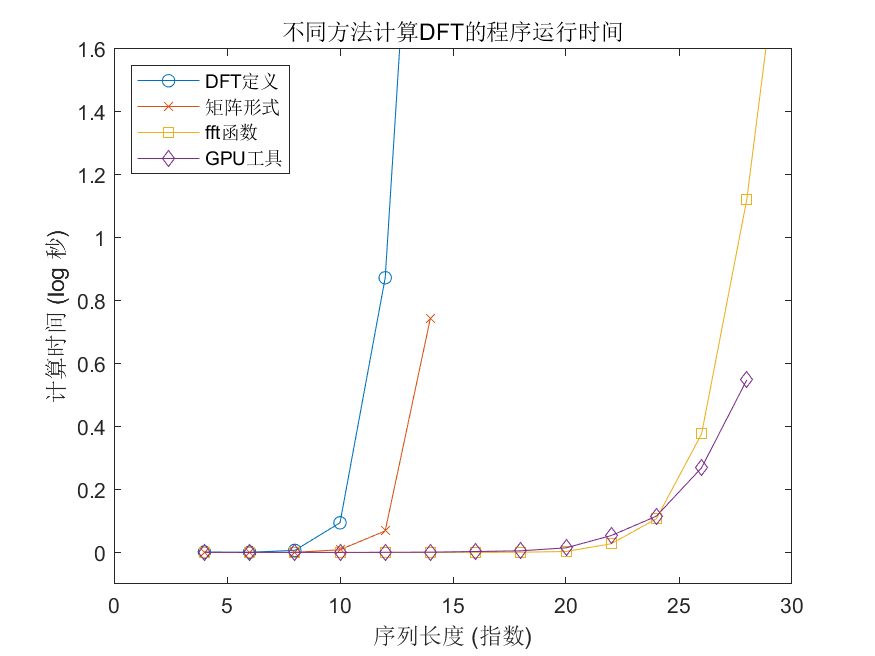
\includegraphics[width=0.75\textwidth]{../code/NVIDIA GeForce RTX 4090}
		\caption{一号机结果 }
	\end{figure}

	一号机：Intel Core i7-13700K 64GDDR5 NVIDIA GeForce RTX 4090 24G Window11
	
	\begin{figure}[h!]
		\centering
		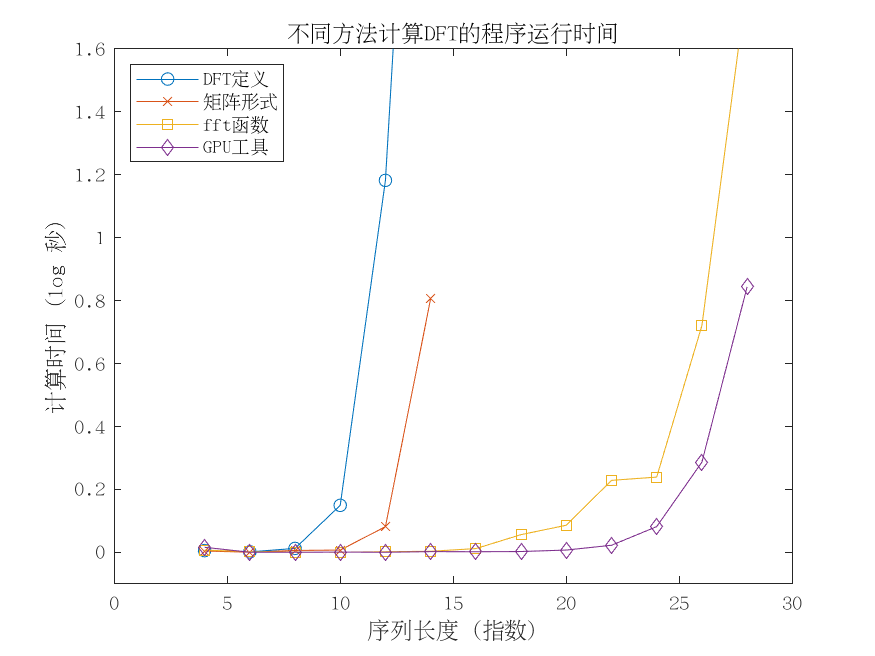
\includegraphics[width=0.75\textwidth]{../code/NVIDIA GeForce RTX 2080 Ti NVIDIA GeForce RTX 2080 Ti}
		\caption{二号机结果}
	\end{figure}

	二号机：AMD Threadripper 2950X 64GDDR4 NVIDIA GeForce RTX 2080Ti*2 22G Ubuntu22.04
\end{document}